% !TEX encoding = UTF-8 Unicode
% !TEX root =  ../Bachelorarbeit.tex

%++++++++++++++++++++++++++++++++++++++++++++++++++++++++++++++++++++++++++++++++++++++++++++++++++++%

\chapter{Entwicklung}
\label{cha:Entwicklung}

Aufbauend auf den in den vorangegangenen Kapiteln -- \Kapitel{TIMER&ISR} und \Kapitel{eUSCI} -- vermittelten theoretischen Grundlagen zu Timern, Interrupt Service Routinen (ISR) und dem Enhanced Universal Serial Communication Interface des Mikrocontrollers MSP430FR5729, widmet sich dieses Kapitel der Entwicklung und praktischen Umsetzung der interruptgesteuerten Benutzerschnittstelle.

Zun\"achst erfolgt die systematische Konzeptionierung des \glqq Observer-Moduls\grqq. Dieses dient als zentrale Instanz zur Erfassung und Bearbeitung von Befehlseingaben sowie zur Steuerung zugeh\"origer Systemausgaben. Dieses Modul stellt somit die Grundlage f\"ur die Interaktion zwischen Benutzer und Mikrocontroller dar.

Im weiteren Verlauf wird die Konfiguration der interruptgesteuerten Kommunikation \"uber die UART-Schnittstelle erarbeitet. Hierbei liegt der Fokus auf zuverl\"assigkeit und robustheit sowie deren sicherer Ausgabe unter Echtzeitbedingungen.

Abschlie{\ss}end werden zentrale Debugging-Mechanismen vorgestellt, evaluiert und exemplarisch in Form von softwarebasierten Breakpoints implementiert. Ziel ist es, die Robustheit, Echtzeitf\"ahigkeit sowie den funktionalen Umfang der zu entwickelnden Komponente zu validieren und zu evaluieren.

Die Integration von Breakpoints erm\"oglicht es, gezielt in den Programmablauf eingreifen zu k\"onnen, ohne den Systemzustand zu beeintr\"achtigen. Insbesondere zu integrierende Funktionen f\"ur das lesen und beschreiben von Speicherzellen profitieren hiervon. Wird ein Breakpoint erreicht, k\"onnen diese Befehle kontrolliert und st\"orungsfrei ausgef\"uhrt werden, da das Hauptprogramm w\"ahrenddessen in einen definierten Haltemodus versetzt wird. Auf diese Weise l\"asst sich eine konsistente Speicherzugriffslogik realisieren, die auch w\"ahrend kritischer Zust\"ande wie Kontextwechsel zuverl\"assig funktioniert.\AI

%====================================================================================================%

\newpage
\section{Konzeprionierung Observer-Modul}
\label{sec:ObserverModulKonzept}

Die zentrale Einheit zur Verarbeitung eingehender Befehle und zur Steuerung s\"amtlicher Funktionen stellt das Observer-Modul dar. Es vereint die Interrupt-Basierte Abarbeitung sowie das Senden von Daten und Empfang externer Steuerbefehle. Die im \Kapitel{TIMER&ISR} und \Kapitel{eUSCI} erl\"auterten Technologien des MSP430FR5729 bilden hierzu die technische Grundlage.

Alle gew\"unschten Komponenten und ihre funktionale Zuordnung ist in \Abbildung{UmlDiagram_ObserverModul} zusammengefasst.

\begin{figure}[h!]
	\centering
	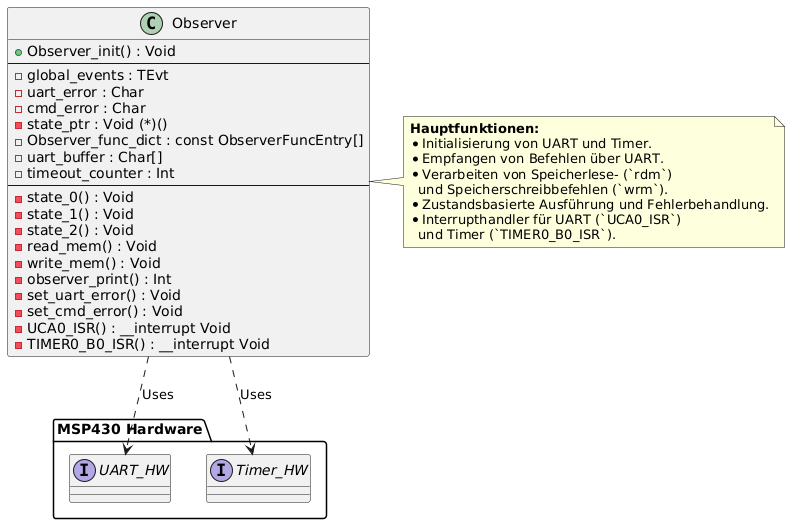
\includegraphics[width=1.0\textwidth]{../Bilder/observer_class_diagram.png}
	\caption{UML-Diagram -- Observer-Modul}
	\label{fig:UmlDiagram_ObserverModul}
\end{figure}

Ausgehend vom grundlegenden Architekturkonzept des Observer-Moduls erfolgt in einem kommenden Kapitel -- \Kapitel{Interruptgesteuertes_Lesen&Schreiben} -- eine detaillierte erkl\"arung der Implementierung der Funktionen f\"ur das interruptgesteuerte Lesen und Schreiben \"uber die serielle Schnittstelle.

%----------------------------------------------------------------------------------------------------%

\newpage
\subsection{Zustandsautomat und Funktionsumfang}
\label{sec:ZustaendeUndFunktionen}

Der Programmablauf, nach der Initialisierung des Moduls bis zur erfolgreichen Ausgabe einer Information, beschreibt sich wie folgt:
Solange kein Befehl \"uber die Eingabetaste eines verbundenen PCs best\"atigt wurde, verbleibt das Modul im Ruhezustand. Bereits ab dem ersten \Fachbegriff{Zeichenkombination aus Buchstaben (lateinisches Alphabet) und Ziffern (0–9)}{alphanumerischen}[alphanumerisch] Zeichen wird ein \glqq Time-Out\grqq-Timer aktiviert. Dieser Time-Out-Timer bildet den ersten von drei Zust\"anden (\Code{state\_0}). Erfolgt innerhalb eines definierten Zeitintervalls keine abschlie{\ss}ende Eingabe, wird der Vorgang \"uber den Zustand \Code{state\_2} zur\"uckgesetzt, und es wird ein \glqq Time-Out-Error\grqq generiert. bei erfolgreicher Best\"atigung hingegen wird der Timer deaktiviert und \"uber den Zustand \Code{state\_1} die Befehlsinterpretation eingeleitet. In \Code{state\_1} wird ein zum Befehl passender Funktionszeiger dem Statuszeiger zugewiesen. Das Ergebnis der Befehlsverarbeitung wird anschlie{\ss}end \"uber UART zur\"uckgegeben. Etwaige Fehler im Ablauf werden mithilfe eines Fehlervektors priorisiert, gespeichert und entsprechend ausgegeben. Das Observer-Modul arbeitet statusorientiert und verarbeitet Ereignisse gem\"a{\ss} ihres Auftretens. \Abbildung{StateMachine_ObserverModul} zeigt einen voll Umfassenden \Fachbegriff{Auch endlicher Automat, ist ein mathematisches Modell zur Beschreibung von Systemen mit endlich vielen Zust\"anden, das \"Uberg\"ange zwischen diesen in Abh\"angigkeit von Eingaben definiert.}{Zustandsautomaten}[Zustandsautomat].
Eine detaillierte Beschreibung der Abarbeitung gesetzter Zust\"ande findet sich in \Kapitel{Timer_ISR}.

\begin{figure}[h!]
	\centering
	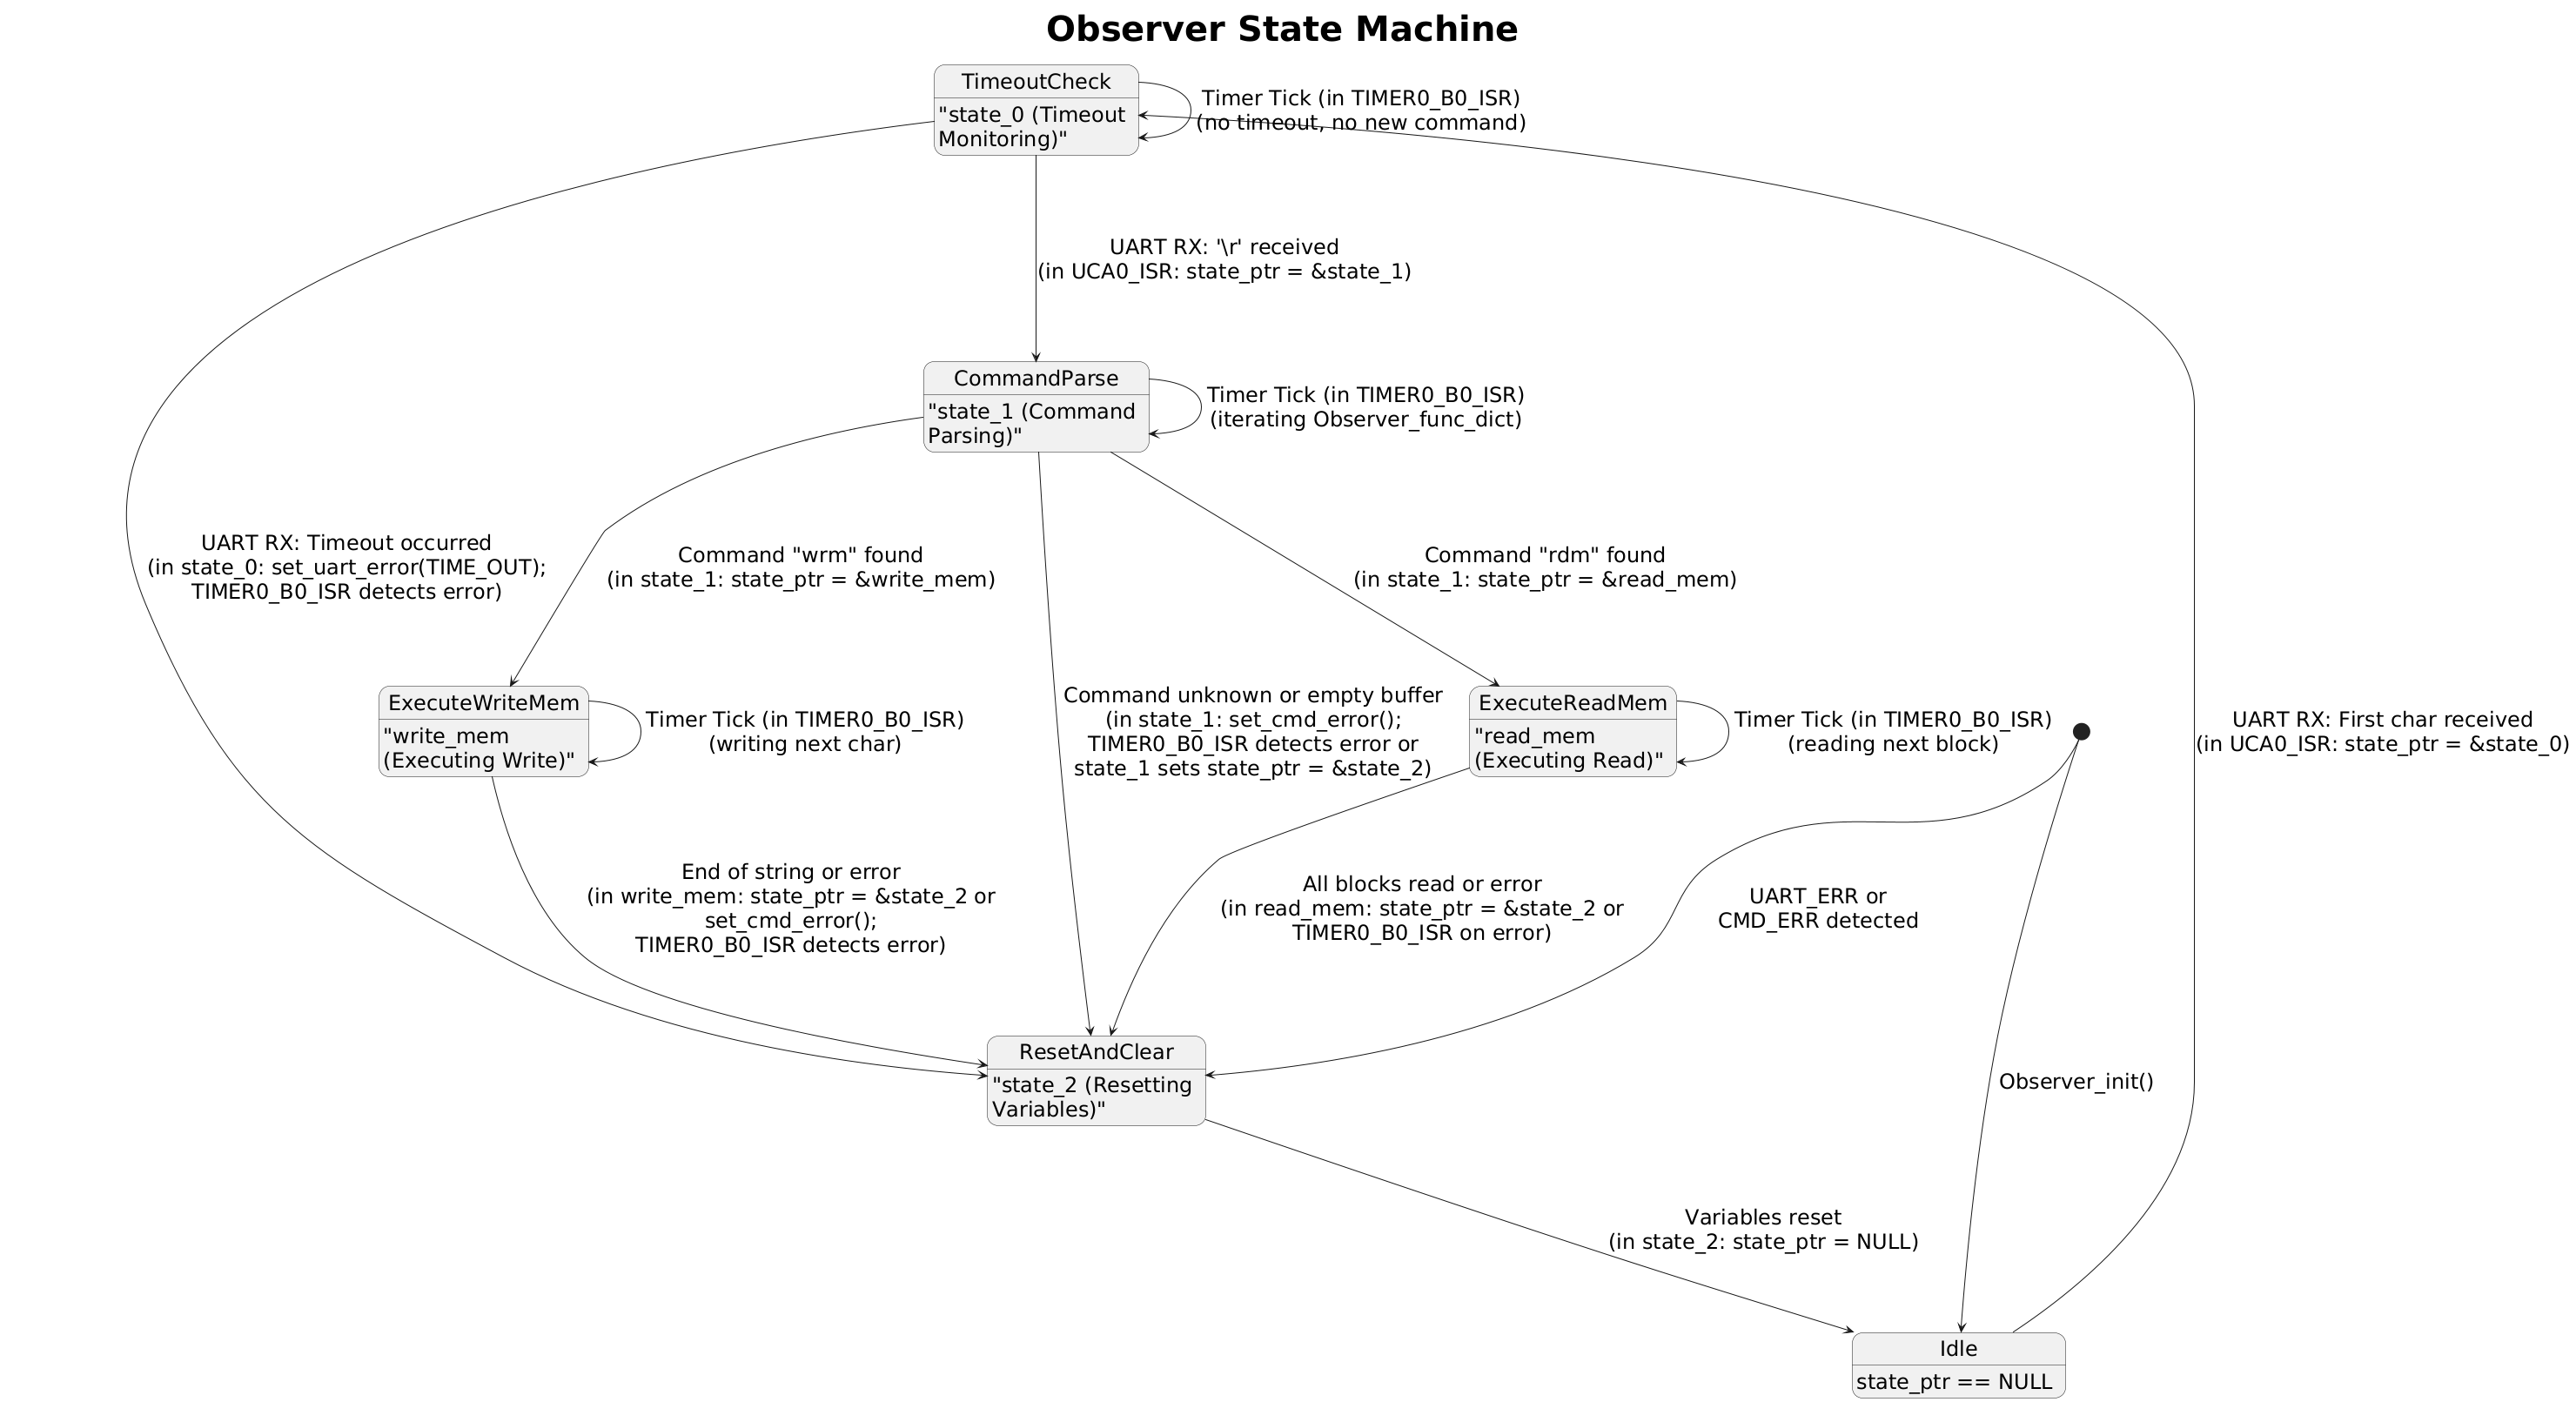
\includegraphics[width=1.0\textwidth]{../Bilder/observer_state_machine.png}
	\caption{Zustandsautomat -- Observer-Modul}
	\label{fig:StateMachine_ObserverModul}
\end{figure}

%----------------------------------------------------------------------------------------------------%

\newpage
\subsection{Initialisierung}
\label{sec:Init}

Ein funktionales Modul, welches die daf\"ur ben\"otigten Hardware-Komponenten – insbesondere Interrupt Service Routines (ISR) und das eUSCI-Modul – integriert, erfordert eine \"offentlich zug\"angliche Initialisierungsmethode, die von der Hauptroutine aufgerufen wird. Diese Methode \"ubernimmt die Konfiguration der Steuerregister sowie die Initialisierung ben\"otigter Variablen und Datenstrukturen.

F\"ur die Ein- und Ausgabe \"uber UART kann die in \Kapitel{eUSCI_Konfiguration} beschriebene Konfiguration \"ubernommen werden. Folgende Einstellungen haben sich dabei als vorteilhaft erwiesen:

\begin{itemize}
	\item Gerade Parit\"at
	\item LSB-first
	\item Acht-Datenbits
	\item Ein Stoppbit
	\item UART-Modus
	\item Asynchroner Modus
	\item ACLK-Taktquelle
	\item Aktiver Fehler-Interrupt
	\item Aktiver Break-Interrupt
	\item 9600 Baud
	\item 16-faches Oversampling
	\item Entprellzeit von rund 100ns
\end{itemize}

Die Verarbeitung von Ereignissen wie Befehlsinterpretation, Fehlerausgabe und Eingabe-Time-Out wird \"uber eine gemeinsame ISR realisiert. Eine daf\"ur passende Periodendauer betr\"agt 10\,ms. \Kapitel{TIMER&ISR} beschreibt die verf\"ugbaren Timer des MSP430FR5729. Aufgrund der in diesem Zusammenhang dargestellten Eigenschaften erweist sich ein Timer vom Typ B als besonders geeignet, da seine erweiterte Konfiguration -- gegen\"uber des Timers von Typ A -- eine skalierbare und anpassungsf\"ahige Implementierung des Moduls im Hinblick auf zuk\"unftige Systemanforderungen erlaubt. Neben den funktionalen Vorteilen ergibt sich die Wahl des Timers auch deshalb, weil im System bereits s\"amtliche Timer vom Typ A anderweitig genutzt werden.

Die relevante Konfiguration der Capture-/Compare-Register basiert auf folgenden Parametern:

\begin{itemize}
	\item Compare-Modus
	\item UP-Modus
	\item ACKL als Taktquelle
	\item Input Teiler jeweils auf acht
	\item Compare-Register auf 96 setzen
	\item Aktivierter Timer-Interrupt
\end{itemize}

Der Wert f\"ur das Compare-Register ergibt sich aus folgender Formel:

\[
\text{Compare-Wert} = \frac{f_\text{ACLK} \cdot T_\text{Periode}}{\text{Teiler}_1 \cdot \text{Teiler}_2} = \frac{614{,}4\,\text{kHz} \cdot 10\,\text{ms}}{8 \cdot 8} = 96
\]

Weitere Initialisierungen umfassen:
\begin{itemize}
	\item Puffervariablen zur Zeichenspeicherung,
	\item Event- und Fehlerflags,
	\item Laufvariablen und Zeiger zur schnellen Navigation innerhalb von Eingabepuffern,
	\item sowie Funktionszeiger f\"ur die Ereignisverarbeitung.
\end{itemize}

Ein besonderer Vorteil ergibt sich durch den Einsatz eines \Fachbegriff{Datenstruktur, die Schl\"ussel-Wert-Paare speichert und schnellen Zugriff auf Werte \"uber ihre eindeutigen Schl\"ussel erlaubt.}{Dictionarys}[Dictionary], das Befehlen eindeutig Funktionszeiger zuordnet.

%----------------------------------------------------------------------------------------------------%

\newpage
\subsection{Timer ISR}
\label{sec:Timer_ISR}

Dieses Unterkapitel thematisiert die Timer-ISR innerhalb des Observer-Moduls. Funktionen im Hinblick auf die Fehlerbehandlung und die Steuerung der Zustandslogik sind dar\"uber Implementiert.

Die Timer-ISR wird periodisch ausgef\"uhrt und fungiert als fundamentaler Taktgeber f\"ur die operativen Sequenzen des Moduls. Die Frequenz dieses Taktes bestimmt die Reaktionsgeschwindigkeit des Systems auf sowohl externe Ereignisse als auch interne Prozesse. Darunter f\"allt der Abschluss einer Befehlseingabe oder die Evaluierung und Signalisierung von Fehlerzust\"anden. Um die Leistung und Reaktivit\"at nicht negativ zu beeintr\"achtigen, ist der Programmcode innerhalb dieser ISR bewusst minimal und ist auf Ausf\"uhrungszeit optimiert. Diese Ma{\ss}nahme ist kritisch, da Interrupts naturgem\"a{\ss} eine blockierende Wirkung auf den Prozessfluss haben.

Der Ablauf der Timer-ISR ist im Aktivit\"atsdiagramm in \Abbildung{activity_diagram_timer_isr} detailliert dargestellt. Die ISR wird durch das Setzen des TBIFG-Flags im TB0CTL-Register des Timer B0 ausgel\"ost, nachdem dieser den in TB0CCR0 definierten Z\"ahlwert erreicht hat. Ausf\"uhrlicher in \Kapitel{CC_Register} und \Kapitel{TimerControlRegister} besprochen. Die prim\"aren Aufgaben der Timer-ISR umfassen:

\begin{itemize}
	\item \textbf{Fehlerbehandlung und -signalisierung:} Bei Eintritt pr\"uft die ISR den globalen Ereignis-Parameter -- \Code{global\_events} -- auf eine registrierte UART- (\Code{UART\_ERR}) oder Befehls-Fehler-Flag (\Code{CMD\_ERR}). Wird ein Fehler detektiert, initiiert die Routine die Ausgabe der dazugeh\"origen Fehlermeldung \"uber die UART-Schnittstelle mittels der Funktion \Code{observer\_print}, welche in \Listing{observer_print} aus \Kapitel{label} dargestellt ist. Anschlie{\ss}end wird die entsprechende Fehler-Flag zur\"uckgesetzt und der Zustands-Funktionszeiger \Code{state\_ptr} auf die Reset-Funktion \Code{state\_2} gesetzt, um das Modul in einen definierten Ausgangszustand zu \"uberf\"uhren.

	\item \textbf{Ausf\"uhrung der Zustandslogik:} Sofern keine Fehlerbehandlung aktiv ist, wird die durch den Funktionszeiger \Code{state\_ptr} referenzierte Zustandsfunktion aufgerufen. Dies erm\"oglicht die schrittweise Abarbeitung implementierter Zust\"ande. Mehr dazu in \Kapitel{Interruptgesteuertes_Lesen&Schreiben}.
\end{itemize}

Abschlie{\ss}end wird das \Code{TBIFG}-Interrupt-Flag im \Code{TB0CTL}-Register gel\"oscht, um die ISR f\"ur den n\"achsten Zyklus vorzubereiten. Die periodische Natur dieser Routine ist essentiell f\"ur weitere Funktionen wie die Timeout-Erkennung bei der Befehlseingabe und die nicht-blockierende Ausf\"uhrung l\"angerer Operationen.

\begin{figure}[h!]
	\centering
	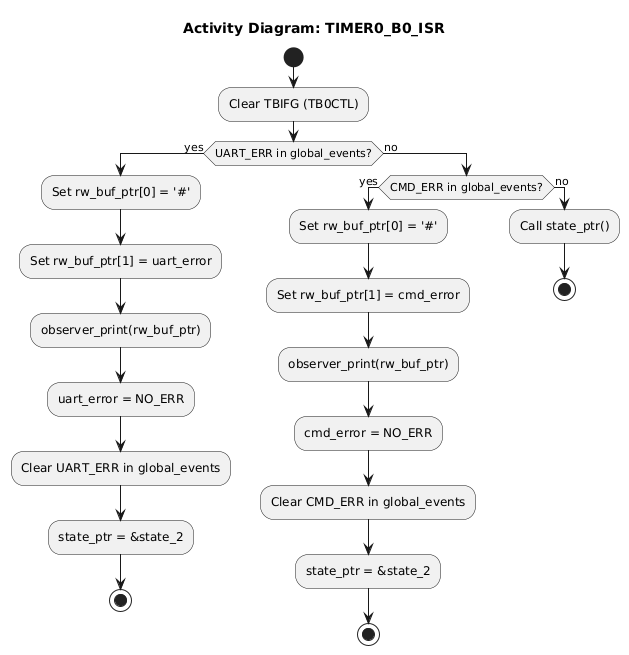
\includegraphics[width=0.50\textwidth]{../Bilder/observer_activity_diagram_timer_b0.png}
	\caption{Aktivit\"atsdiagramm -- Timer ISR}
	\label{fig:activity_diagram_timer_isr}
\end{figure}

%----------------------------------------------------------------------------------------------------%

\newpage
\subsection{UART ISR}
\label{sec:UART_ISR}

Eine weitere unerl\"assliche Komponente des Observer-Moduls ist die Interrupt Service Routine der UART-Kommunikation. Diese steuert den bidirektionalen Datenaustausch, \dahe das Senden und Empfangen von Zeichen \"uber die serielle Schnittstelle. Sie behandelt zudem Grenzf\"allen, wie den Empfang ung\"ultiger Zeichen oder spezifische UART-Fehlerzust\"ande. Im Unterschied zur zyklisch operierenden Timer-ISR (siehe \Kapitel{Timer_ISR}) wird die UART-ISR ereignisgesteuert ausgel\"ost: entweder nach dem Empfang eines Datenbytes im Empfangspuffer (\Code{UCA0RXBUF}) oder wenn der Sendepuffer (\Code{UCA0TXBUF}) bereit ist, ein neues Datenbyte f\"ur die \"ubertragung aufzunehmen. Die Unterscheidung zwischen den verschiedenen UART-Ereignissen -- wie \zB Empfangen, Senden oder Fehler erkannt -- erfolgt \"uber das Interrupt-Vektor-Register \Code{UCA0IV}. Tiefgreifendere Informationen dar\"uber in \Kapitel{datenintegritaet} und \Kapitel{eUSCI_Zusammenfassung}.

Die Empfangslogik -- definiert \"uber den Interruptvektor \Code{USCI\_UART\_UCRXIFG} -- der UART-ISR l\"asst sich anhand des Aktivit\"atsdiagramms in \Abbildung{activity_diagram_uart_isr_rec} pr\"azise nachvollziehen. Zu den Kernaufgaben des Empfangsteils z\"ahlen:

\begin{itemize}
	\item \textbf{Fehlerdetektion:} Pr\"ufung auf Kommunikationsfehler wie \Code{UCBRK} (Break-Signal) oder \Code{UCRXERR} (Framing-, Overrun- oder Parit\"atsfehler) und entsprechendes Setzen eines UART-Fehler-Wertes -- in der \Code{uart\_error}-Variable. 
	
	\item \textbf{Zeichenbehandlung:} Verarbeitung empfangener Bytes -- und zwischenspeichern in der \Code{rx\_byte}-Variable --, inklusive spezieller Steuerzeichen wie \grqq \texttt{\textbackslash r}\grqq (Carriage Return), das die Befehlseingabe abschlie{\ss}t und die Zustandsmaschine aktiviert, sowie \grqq \texttt{\textbackslash b}\grqq (Backspace) zur Korrektur von Eingaben im \Code{uart\_buffer}, und \grqq \texttt{\textbackslash n}\grqq (Newline), das ignoriert wird.

	\item \textbf{Pufferverwaltung:} Validierung (Pr\"ufung auf Alphanumerik und Leerzeichen), Pufferung der g\"ultiger Zeichen im uart\_buffer inklusive \"uberlaufschutz und Echo-Ausgabe des Zeichens.

	\item \textbf{Timeout-Initiierung:} Bei Empfang des ersten Zeichens nach einem Reset wird \Code{state\_ptr} auf \Code{state\_0} gesetzt, welches die Timeout-\"Uberwachung startet.
\end{itemize}

\newpage
\begin{figure}[h!]
	\centering
	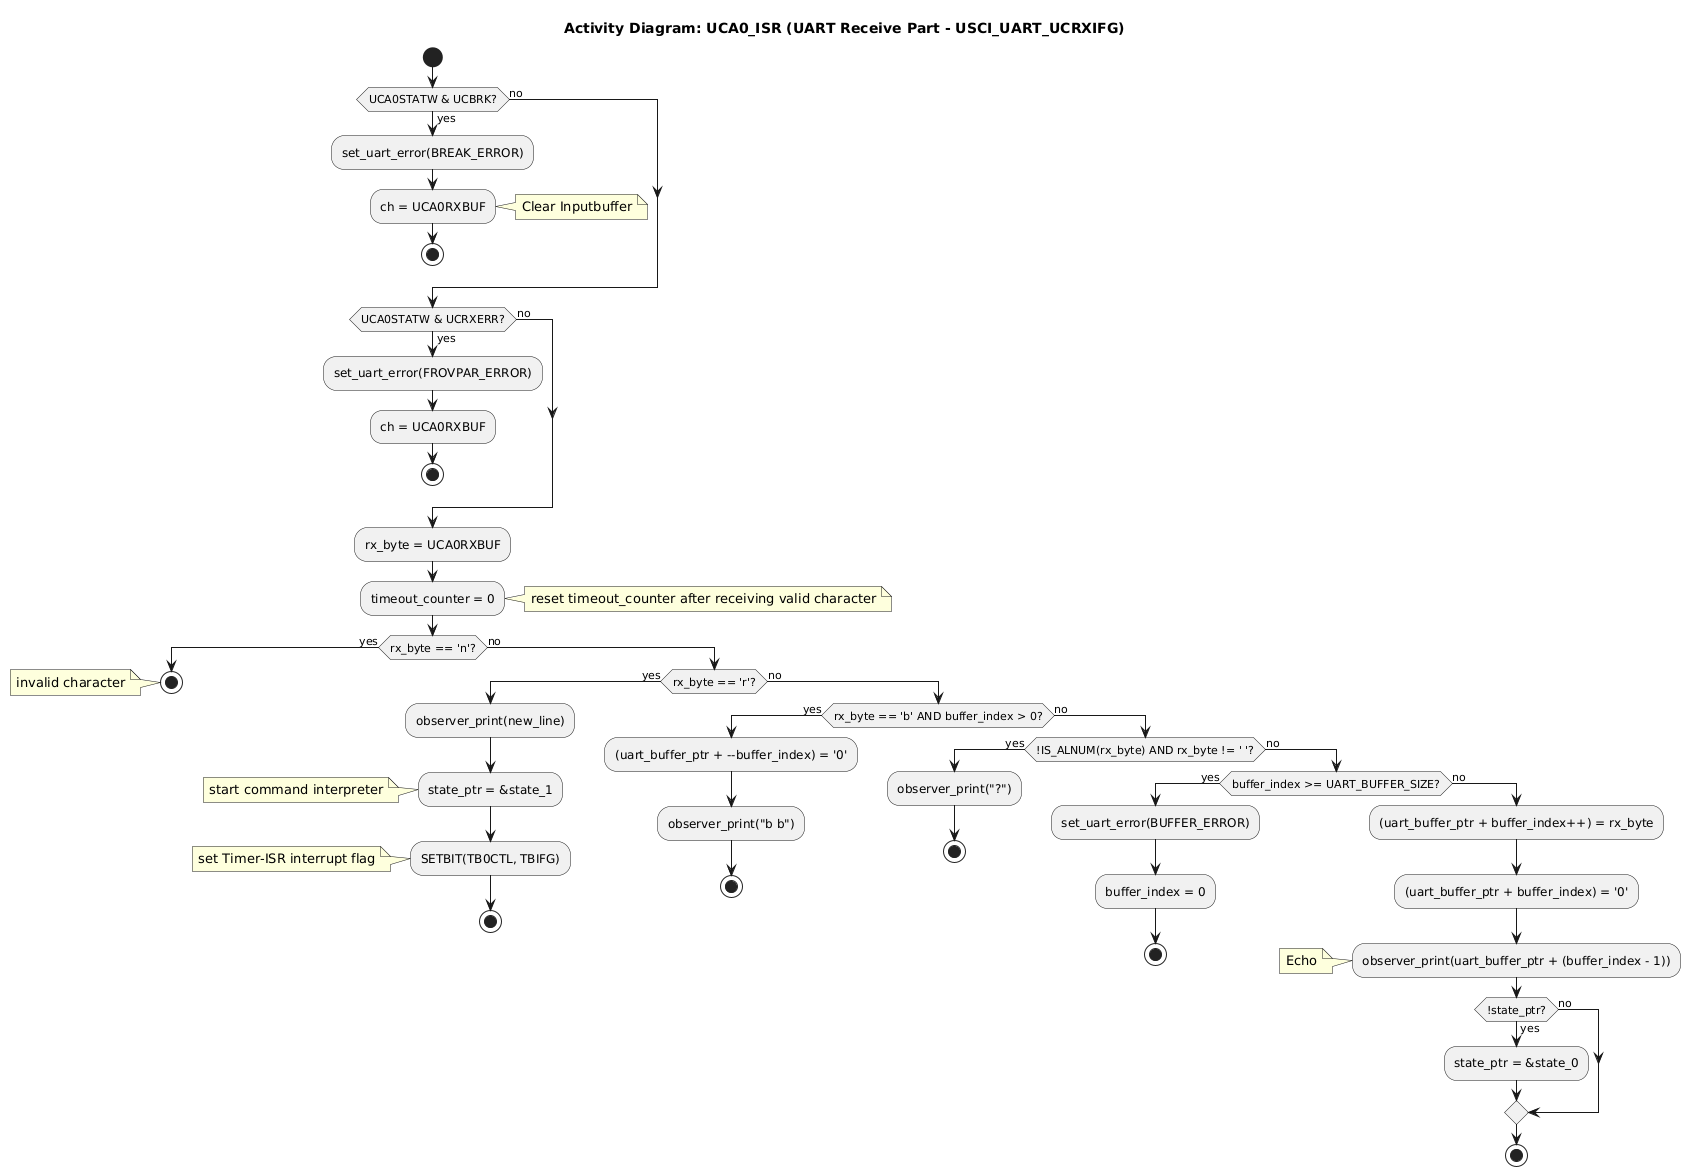
\includegraphics[angle=270, width=1.0\textwidth]{../Bilder/observer_activity_diagram_eusci_receive.png}
	\caption{Aktivit\"atsdiagramm -- Timer ISR}
	\label{fig:activity_diagram_uart_isr_rec}
\end{figure}

\newpage
Der Sendeteil -- mit dem Interruptvektor \Code{USCI\_UART\_UCTXIFG} -- der UART-ISR, dessen Ablauf in \Abbildung{activity_diagram_uart_isr_send} visualisiert ist, ist f\"ur die schrittweise Ausgabe von Zeichenketten zust\"andig. Solange \Code{print\_ptr} nicht auf ein Null-Terminierungszeichen (\grq \texttt{\textbackslash 0}\grq) zeigt, wird das aktuelle Zeichen in den Sendepuffer \Code{UCA0TXBUF} geladen. Nach erfolgreicher \"ubertragung aller Zeichen einer Nachricht wird das \Code{WRT\_UART}-Flag in \Code{global\_events} zur\"uckgesetzt und der Sendeinterrupt (\Code{UCTXIE}) deaktiviert, w\"ahrend der Empfangsinterrupt (\Code{UCRXIE}) reaktiviert wird. Diese ISR ist somit die direkte Schnittstelle f\"ur alle von \Code{observer\_print} initiierten Schreibvorg\"ange.

\begin{figure}[h!]
	\centering
	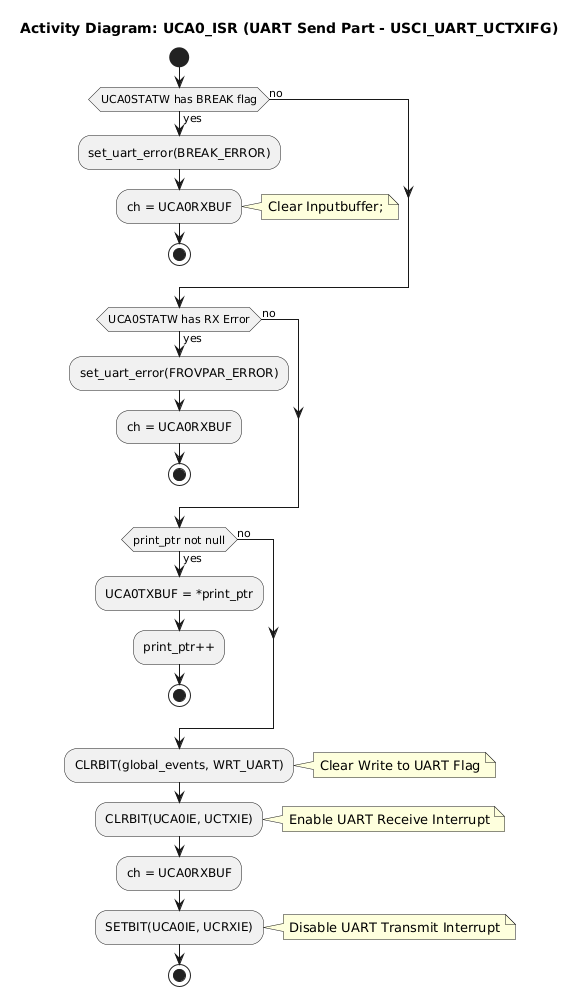
\includegraphics[width=0.60\textwidth]{../Bilder/observer_activity_diagram_eusci_send.png}
	\caption{Aktivit\"atsdiagramm -- Timer ISR}
	\label{fig:activity_diagram_uart_isr_send}
\end{figure}

\newpage
Die zuvor erw\"ahnte \Code{observer\_print}-Funktion dient der Initialisierung eines asynchronen Zeichenkettenausgabevorgangs \"uber eine UART-Schnittstelle. Zun\"achst \"uberpr\"uft sie, ob der \"ubergebene String-Zeiger \Code{str} \Code{null} ist, was auf einen ung\"ultigen Eingabewert hinweist; in diesem Fall wird ein Fehlerstatus gesetzt und der Vorgang abgebrochen. Andernfalls wird eine globale Ereignis-Flagge (\Code{WRT\_UART}) gesetzt, das die UART-\"Ubertragung signalisiert. Der Zeiger auf die zu \"ubertragende Zeichenkette wird in die globale Variable \Code{print\_ptr} geschrieben, woraufhin durch Setzen der Interrupt-Flags \Code{UCTXIFG} und \Code{UCTXIE} der UART-Sendeinterrupt aktiviert wird. Dadurch wird der eigentliche \"Ubertragungsvorgang vom Interrupt-Handler durchgef\"uhrt, was eine nicht-blockierende Daten\"ubertragung erm\"oglicht.

\vspace{0.5cm}
\begin{lstlisting} [style=modernC, caption={Initiierungs-Funktion für UART Daten\"ubertragung}, label={lst:observer_print}]
	#pragma FUNC_ALWAYS_INLINE(observer_print)
	LOCAL Void observer_print(const char * str) {
		if (str EQ NULL) {
			set_uart_error(PRINT_ERROR);
			return;
		}
		SETBIT(global_events, WRT_UART);
		print_ptr = str;
		SETBIT(UCA0IFG, UCTXIFG);   // UART Transmit Interrupt Flag
		SETBIT(UCA0IE,  UCTXIE);    // Enable UART Receive Interrupt
		return;
	}
\end{lstlisting}

%====================================================================================================%

\newpage
\section{Interruptgesteuertes Lesen und Schreiben}
\label{sec:Interruptgesteuertes_Lesen&Schreiben}

Aufbauend auf dem Grundkonzept des Observer-Moduls und der etablierten Architektur lassen sich Funktionalit\"aten und weitere Features integrieren. Im Rahmen dieser Arbeit fiel die Wahl f\"ur eine Kernfunktion auf das interruptgesteuerte Lesen und Schreiben von FRAM-Speicherzellen. Die nachfolgenden Abschnitte erarbeiten die Konzeption und Implementierung dieser Speicheroperationen und analysieren potenzielle Limitationen. Ein fundamentales Merkmal hierbei ist, dass die interruptgesteuerten Speicherzugriffe nicht zwingend einen expliziten Haltezustand des Gesamtsystems erfordern –- wie im Kontext der m\"oglichen Debugging-Funktion in \Chapter{Entwicklung} erl\"autert. Die angestrebte Funktionalit\"at kann auch ohne diese Art an erweiterte Systemkontrolle, eigenst\"andig agieren. Ein potenzieller Nachteil dessen ist jedoch in der Datenkonsistenz der Ausgabe: Durch die zustandsorientierte, inkrementelle Verarbeitung der Lese- und Schreibvorg\"ange k\"onnten konkurrierende Prozesse den adressierten Speicherbereich zwischen einzelnen Verarbeitungsschritten modifizieren. Daraus ergibt sich ein weiterer Grund f\"ur die Notwendigkeit, das Grundkonzept des statusorientierten, interruptgesteuerten Betriebs umzusetzen – wie im Folgenden beschrieben.

%----------------------------------------------------------------------------------------------------%

\subsection{Grundkonzept des statusorientierten, interruptgesteuerten Betriebs}
\label{sec:konzept_status_&_interrupt}

Die zustandsorientierte Programmierung f\"ur das Observer-Modul setzt die Dekomposition komplexer, sequenzieller Abl\"aufe in kleinere, Verarbeitungseinheiten voraus. Wie bereits im \Kapitel{ZustaendeUndFunktionen} und \Kapitel{Timer_ISR} dargelegt, repr\"asentieren die Lese- und Schreiboperationen dedizierte Zust\"ande innerhalb der \"ubergeordneten Zustandsmaschine. Diese Unterteilung ist essentiell, um die Reaktionsf\"ahigkeit des Systems auf externe Eingaben und die parallele Bearbeitung anderer systeminterner Aufgaben sicherzustellen. F\"ur die Realisierung der Speicherzugriffe sind neben generischen Zust\"anden -- zur Befehlsverarbeitung und Systeminitialisierung -- spezifische Zust\"ande f\"ur das Lesen und Schreiben erforderlich. Da diese Operationen, insbesondere bei gr\"o{\ss}eren Speicherzugriffen, potenziell zeitintensiv sind, ist die \"Uberf\"uhrung in eine zeichenorientierte Verarbeitung, welche periodisch durch die Timer-ISR ausgef\"uhrt wird, notwendig.

Konkret bedeutet dies, dass nach der Verarbeitung eines einzelnen Zeichens die jeweilige Speicherroutine tempor\"ar terminiert und die Kontrolle an das System zur\"uckgibt. Die Fortsetzung der Operation erfolgt erst bei der n\"achsten Periode der Timer-ISR. Dieser inkrementelle Ansatz steigert die Reaktivit\"at des Gesamtsystems erheblich. Im Fazit unter \Kapitel{laufzeit} wurden hierzu Laufzeitmessungen unter Realbedingungen durchgef\"uhrt und genauer untersucht. Dem gegen\"uber steht der Nachteil, dass eine zus\"atzliche Laufvariable zum verfolgen des aktuellen Fortschritts, innerhalb der Lese- oder Schreiboperation, ben\"otigt wird. Dadurch entsteht eine potentiell l\"angere Gesamtdauer f\"ur die vollst\"andige Operation ergeben, da pro Timer-Zyklus lediglich ein einzelnes Zeichen verarbeitet wird.\AI

%----------------------------------------------------------------------------------------------------%

\subsection{Rolle der Interrupt Service Routinen}
\label{sec:LesenSchreiben_Rolle_ISR}

Die beiden prim\"aren Interrupt Service Routinen des Moduls, die UART-ISR und die Timer-ISR, erf\"ullen dabei kritische Funktionen im gesamten Prozesszyklus der Speicheroperationen –- von der initialen Befehlseingabe \"uber die schrittweise Datenverarbeitung bis hin zur finalen Ergebnisausgabe.

\begin{itemize}
	\item \textbf{Die UART-ISR:} Agiert als prim\"are Schnittstelle f\"ur die Benutzerinteraktion. Sie ist verantwortlich f\"ur den Empfang vollst\"andiger Befehlsstrings, wie beispielsweise \grqq\Code{rdm <adresse> <bytes>}\grqq, zur Anforderung eines Speicherlesevorgangs oder \grqq\Code{wrm <adresse> <string>}\grqq, zur Initiierung eines Schreibvorgangs. Dar\"uber hinaus \"ubernimmt die UART-ISR die Ausgabe der aus dem FRAM gelesenen Daten an den Benutzer und quittiert einen erfolgreich abgeschlossenen Schreibvorgang durch erneute Ausgabe des Befehls.
	
	\item \textbf{Die Timer-ISR:} Fungiert als periodischer Ausl\"oser und Taktgeber f\"ur die Ausf\"uhrung zustandsbasierter Funktionen. Sie ruft wiederholt die im Funktionszeiger \Code{state\_ptr} referenzierte, aktuell aktive Zustandsfunktion (\zB \Code{read\_mem} oder \Code{write\_mem}) auf. Diese Funktion bleibt so lange aktiv, bis ein definierter Endzustand der jeweiligen Operation erreicht ist.
\end{itemize}

%----------------------------------------------------------------------------------------------------%

\newpage
\subsection{Implementierung der Lese- und Schreibfunktion}
\label{sec:Implementierung_Lesen_Schreiben}

Die softwaretechnische Realisierung der Lese- und Schreibfunktionen ist bewusst ressourcenschonend und auf Laufzeit optimiert. Diese Funktionen besitzen im Wesentlichen einen definierten Startzustand, einen Endzustand sowie die Logik f\"ur den eigentlichen, inkrementellen Speicherzugriff.

Der Programmablauf der \Code{read\_mem}-Funktion ist wie folgt strukturiert (siehe auch Quellcodeausschnitt in \Listing{read_mem_function}):
\begin{itemize}
	\item \textbf{Initiierung:} Die Funktion wird aktiviert, sobald die Befehlsverarbeitungsroutine (\Code{state\_1}) einen \grqq rdm\grqq-Befehl identifiziert und den globalen Zustandszeiger \Code{state\_ptr} auf die Adresse der \Code{read\_mem}-Funktion setzt. Gleichzeitig werden die f\"ur den Lesevorgang notwendigen Parameter –- die Startadresse (gespeichert in \Code{mem\_addr\_ptr}) und die Anzahl der zu lesenden Bytes (\Code{blocks}) –- aus dem \Code{uart\_buffer} extrahiert und in globalen Variablen zwischengespeichert.
	
	\item \textbf{Inkrementelle Ausf\"uhrung:} Bei jedem Aufruf durch die Timer-ISR wird exakt ein Byte aus dem FRAM an der aktuellen Adresse (\Code{mem\_addr\_ptr + mem\_addr\_idx}) gelesen. Der Fortschritt innerhalb des adressierten Speicherbereichs wird mittels der Indexvariable \Code{mem\_addr\_idx} verfolgt, welche nach jedem gelesenen Byte inkrementiert wird.
	
	\item \textbf{Datenausgabe:} Das eingelesene Zeichen wird einer Validierung unterzogen (Filterung nicht-alphanumerischer Zeichen, die durch Leerzeichen ersetzt werden) und anschlie{\ss}end im Puffer \Code{rw\_buf} abgelegt. Mittels der Zuweisung \grq\Code{print\_ptr = rw\_buf\_ptr}\grq und setzen der Bits f\"ur das senden von Daten \"uber das UART-Protokoll erfolgt die unmittelbare Ausgabe des gelesenen Zeichens an die Benutzerkonsole.
	
	\item \textbf{Beendigung:} Die Leseoperation gilt als abgeschlossen, sobald der Z\"ahler \Code{mem\_addr\_idx} die vorgegebene Anzahl an zu lesenden Bytes erreicht oder \"uberschritten hat. In diesem Fall wird der \Code{state\_ptr} auf den Zeiger der \Code{state\_2}-Funktion (R\"ucksetz- und Leerlaufzustand) umgelenkt, um das System f\"ur neue Befehle vorzubereiten.
\end{itemize}

\newpage
\begin{lstlisting} [style=modernC, caption={Implementierungsausschnitt der \Code{read\_mem}-Funktion im Observer-Modul}, label={lst:read_mem_function}]
	#pragma FUNC_ALWAYS_INLINE(read_mem)
	LOCAL Void read_mem(Void) {
		
		//SETBIT(P3OUT, BIT4);
		if (TSTBIT(global_events & WRT_UART, WRT_UART)) {
			//CLRBIT(P3OUT, BIT4);
			return;
		}
		
		if (mem_addr_idx > (blocks - 1)) {
			state_ptr = &state_2;
			//CLRBIT(P3OUT, BIT4);
			return;
		}
		
		if (mem_addr_ptr EQ NULL) {
			// Extract useful arguments
			Char *mem_addr_str = strtok(uart_buffer_ptr + 4, " ");
			Char *block_str = mem_addr_str + strlen(mem_addr_str) + 1;
			
			mem_addr_ptr = (Char *)strtol(mem_addr_str, NULL, 0);
			blocks = (UInt)atoi(block_str);
		}
		
		*rw_buf_ptr = *((volatile Char *)mem_addr_ptr + mem_addr_idx);
		if (!IS_ALNUM(*rw_buf_ptr)) {
			*rw_buf_ptr = ' ';
		}
		
		print_ptr = rw_buf_ptr;
		SETBIT(global_events, WRT_UART);
		SETBIT(UCA0IFG, UCTXIFG);   // UART Transmit Interrupt Flag
		SETBIT(UCA0IE,  UCTXIE);    // Enable UART Receive Interrupt
		
		mem_addr_idx++;
		
		//CLRBIT(P3OUT, BIT4);
	}
\end{lstlisting}

\newpage
Analog dazu ist der Programmablauf der \Code{write\_mem}-Funktion konzipiert (siehe Quellcodeausschnitt in \Listing{write_mem_function}):
\begin{itemize}
	\item \textbf{Initiierung:} Die Aktivierung erfolgt, wenn die Befehlsverarbeitung (\Code{state\_1}) einen \grqq wrm\grqq-Befehl erkennt und \Code{state\_ptr} auf die \Code{write\_mem}-Funktion setzt. Die Zieladresse (\Code{mem\_addr\_ptr}) und der zu schreibende String (\Code{write\_str\_ptr}) werden aus dem \Code{uart\_buffer} extrahiert.
	
	\item \textbf{Adressvalidierung:} Vor dem eigentlichen Schreibzugriff wird \"uberpr\"uft, ob die angegebene Zieladresse in potenziell schreibgesch\"utzten oder f\"ur andere Zwecke reservierten Speicherbereichen liegt (\zB im Hexadezimalbereich von 0x000000 bis 0x0001FF oder 0x000C00 bis 0x000FFF, mehr Informationen dazu in \Abbildung{memory_map}). Bei Detektion einer ung\"ultigen Adresse wird ein entsprechender Fehlercode (\Code{INV\_ADDR}) gesetzt und die Operation terminiert.
	
	\begin{figure}[h!]
		\centering
		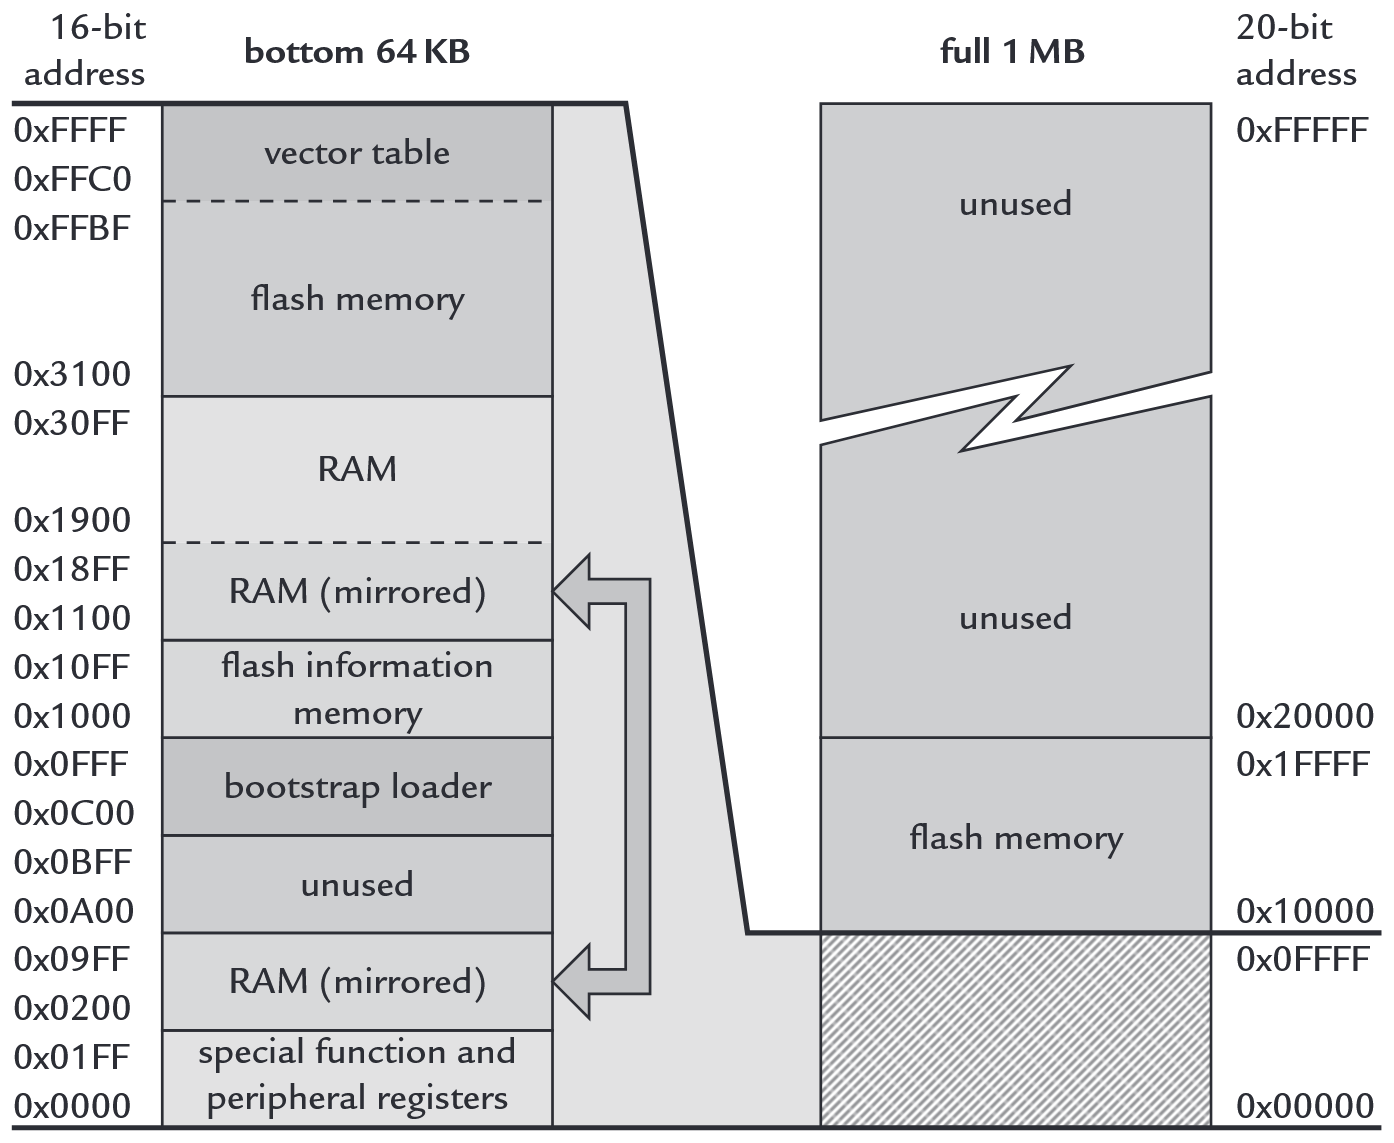
\includegraphics[width=0.75\textwidth]{../Bilder/memory_map.png}
		\caption{Memory map des FG4618 \Zitat[S. 603, Fig. 11.1]{davies:msp430}}
		\label{fig:memory_map}
	\end{figure}
	
	\item \textbf{Inkrementelle Ausf\"uhrung:} Bei jedem Aufruf durch die Timer-ISR wird ein einzelnes Zeichen aus dem \Code{write\_str\_ptr} (an der durch \Code{mem\_addr\_idx} indizierten Position) in die entsprechende FRAM-Speicherzelle (\Code{mem\_addr\_ptr + mem\_addr\_idx}) geschrieben. Der Fortschritt wird durch das hochz\"ahlen der \Code{mem\_addr\_idx}-Variable verfolgt.
	
	\item \textbf{Datenausgabe/Echo:} Das soeben geschriebene Zeichen wird zur Verifikation in den \Code{rw\_buf} kopiert und mittels \Code{observer\_print} als Echo an den Benutzer zur\"uckgesendet.
	
	\item \textbf{Beendigung:} Die Schreiboperation ist abgeschlossen, sobald das Null-Terminierungszeichen (\grq \texttt{\textbackslash 0}\grq) des \Code{write\_str\_ptr} erreicht wurde. Daraufhin wird abermals der \Code{state\_ptr} auf die \Code{state\_2}-Funktion gesetzt, um den Schreibzyklus ordnungsgem\"a{\ss} zu beenden und das Modul in seinen definierten Ausgangszustand zur\"uck zu setzen.
\end{itemize}


\vspace{0.5cm}
\begin{lstlisting} [style=modernC, caption={Implementierungsausschnitt der \Code{write\_mem}-Funktion im Observer-Modul}, label={lst:write_mem_function}]
	#pragma FUNC_ALWAYS_INLINE(write_mem)
	LOCAL Void write_mem(Void) {
		
		//SETBIT(P3OUT, BIT4);
		if (TSTBIT(global_events & WRT_UART, WRT_UART)) {
			//CLRBIT(P3OUT, BIT4);
			return;
		}
		
		if (mem_addr_ptr EQ NULL) {
			// Extract useful arguments
			Char *mem_addr_str = strtok(uart_buffer_ptr + 4, " ");
			write_str_ptr = mem_addr_str + strlen(mem_addr_str) + 1;
			
			mem_addr_ptr = (Char *)strtol(mem_addr_str, NULL, 0);
		}
		
		if (between("0x000000", mem_addr_ptr, "0x0001FF")
		|| between("0x000C00", mem_addr_ptr, "0x000FFF")) {
			set_cmd_error(INV_ADDR);
			return;
		}
		
		*rw_buf_ptr = *((volatile Char *)write_str_ptr + mem_addr_idx);
		
		if (*rw_buf_ptr EQ '\0') {
			state_ptr = &state_2;
			//CLRBIT(P3OUT, BIT4);
			return;
		}
		
		if (!IS_ALNUM(*rw_buf_ptr)) {
			*rw_buf_ptr = ' ';
		}
		
		print_ptr = rw_buf_ptr;
		SETBIT(global_events, WRT_UART);
		SETBIT(UCA0IFG, UCTXIFG);   // UART Transmit Interrupt Flag
		SETBIT(UCA0IE,  UCTXIE);    // Enable UART Receive Interrupt
		
		*((volatile Char *)mem_addr_ptr + mem_addr_idx) = *rw_buf_ptr;
		mem_addr_idx++;
		
		//CLRBIT(P3OUT, BIT4);
	}
\end{lstlisting}

Die Identifikation, Verarbeitung und Signalisierung potenziell auftretender Fehlerzust\"ande ist ein weiterer unerl\"asslicher Entwicklungsschritt. Dieser Aspekt der Fehlerbehandlung wird im nachfolgenden Kapitel eingehend thematisiert.\AI

%====================================================================================================%

\newpage
\section{Fehlerbehandlung}
\label{sec:Fehlerbehandlung}

Die Identifizierung und Auswertung von Randbedingungen sowie die daran anschlie{\ss}ende Fehlerbehandlung sind grundlegende Bestandteile komplexer Softwareprojekte. F\"ur den Nutzer ist die Ausgabe potenziell auftretender Fehlerzust\"ande von hoher Bedeutung, um eine angemessene Fehlerbehebung einleiten zu k\"onnen. Um eine \"Uberlastung des Nutzers mit redundanten oder niederrangigen Fehlermeldungen -- oder Folgefehlern -- zu vermeiden, ist eine interne Speicherung und anschlie{\ss}ende Priorisierung detektierter Fehler notwendig. 

Die prim\"aren Fehlerquellen innerhalb des Observer-Moduls ist die UART- Kommunikationsschnittstelle sowie die Prozesse der Befehlsinterpretation und -ausf\"uhrung.
\begin{itemize}
	\item \textbf{Die UART-Schnittstelle} besitzt diverse Fehlerindikatoren (Fehlervektoren beschrieben in \Kapitel{eUSCI_Konfiguration}), welche direkt zu Beginn der UART-ISR -- sowohl im Sende- als auch im Empfangsteil -- gepr\"uft werden. Ein zus\"atzlicher Fehlerfall ist die \"uberschreitung eines definierten Zeitlimits (Time-Out) pro Zeichen f\"ur die Befehlseingabe. Bei Erreichen dieses Schwellenwerts wird die laufende Befehlseingabe terminiert, das System auf einen deffinierten Ausgangszustand zur\"uckgesetzt und eine entsprechende Fehlermeldung an die verbundene Benutzerkonsole \"ubermittelt.
	
	\item \textbf{Die Befehlsinterpretation sowie -verarbeitung} kann ebenfalls Fehler und definierte Randbedingungen aufweisen. Hierzu z\"ahlt die Detektion unbekannter Befehle, die Verwendung invalider Speicheradressen (\zB Zugriff auf gesch\"utzte Bereiche, \Vgl \Abbildung{memory_map}), fehlerhafte Zeichenketten oder unzul\"assige Blockgr\"o{\ss}en.
\end{itemize}

\newpage
Die hierf\"ur implementierten Funktionen sind in \Listing{fehlerbehandlung_funktionen} dargestellt. Unterschiedliche Fehlerquellen erfordern dabei eine separate Behandlung und Klassifizierung. 

\vspace{0.5cm}
\begin{lstlisting} [style=modernC, caption={Funktion zur Fehlerpriorisierung und Speicherung sowie Setzen eines globalen \Code{Error}-Flags}, label={lst:fehlerbehandlung_funktionen}]
	#pragma FUNC_ALWAYS_INLINE(set_uart_error)
	LOCAL Void set_uart_error(Char err) {
		if (err == NO_ERR || uart_error < err) {
			uart_error = err;
			SETBIT(global_events, UART_ERR);
		}
	}
	
	#pragma FUNC_ALWAYS_INLINE(set_cmd_error)
	LOCAL Void set_cmd_error(Char err) {
		if (err == NO_ERR || cmd_error < err) {
			cmd_error = err;
			SETBIT(global_events, CMD_ERR);
		}
	}
\end{lstlisting}

Die Fehlerpriorisierung basiert auf in der Header-Datei (\Code{Observer.h}) definierten Makros, die entsprechend ihrer Eskalationsstufe numerisch kodiert sind (\Vgl \Listing{error_vectors}). Mittels eines Vergleichsoperators wird evaluiert, ob ein neu aufgetretener Fehler eine h\"ohere Priorit\"at besitzt als ein bereits intern vermerkter Fehler. Nur wenn dies der Fall ist oder noch kein spezifischer Fehler dieser Kategorie gespeichert wurde, wird der neue Fehler als der aktuell relevanteste behandelt und der bisherige gegebenenfalls \"uberschrieben.

\newpage
\begin{lstlisting} [style=modernC, caption={Definition der Fehler-Makros in der Header-Datei \Code{Observer.h} zur Festlegung der Fehlerpriorit\"aten.}, label={lst:error_vectors}]
	/*
	* UART Error
	*/
	#define NO_ERR              0x00    // no error
	#define TIME_OUT            'A'     // time out
	#define BUFFER_ERROR        'B'     // buffer error (e.g. to many bytes received)
	#define FROVPAR_ERROR       'C'     // frame overrun or parity error
	#define BREAK_ERROR         'D'     // break error (lost communication)
	#define PRINT_ERROR         'E'     // unable to print on UART
	
	/*
	* Command Error
	*/
	#define UNKNOWN_CMD         '1'     // unknown command
	#define INV_PTR             '2'     // Invalid function pointer
	#define INV_ADDR            '3'     // Invalid memory address
	#define INV_BLCK            '4'     // Invalid block-size
	#define INV_STR             '5'     // Invalid string
\end{lstlisting}

Die Konstruktion und Ausgabe der finalen Fehlermeldung obliegt der Timer-ISR. Diese Routine identifiziert den spezifischen Fehlerkontext anhand der zuvor gesetzten Fehlerereignis-Flag im globalen Ereignisregister \Code{global\_events}. Der zugeh\"orige Fehlercode im Fehlerregister \Code{uart\_error} oder \Code{cmd\_error}, zusammen mit einem Pr\"afix-Zeichen (\grq \# \grq) ergibt anschlie{\ss}end die Fehlermeldung. F\"ur die Formatierung der Meldung wird der Lese- und Schreib-Puffer \Code{rw\_buf} genutzt. Dessen Gr\"o{\ss}e ist auf drei Byte initialisiert, um das Pr\"afix-Zeichen, den alphanumerischen Fehlercode-Wert und das Null-Terminierungszeichen aufzunehmen. Die Startadresse dieses Puffers wird im Anschluss der Funktion \Code{observer\_print} \"ubergeben, welche die zeichenweise \"ubertragung der Fehlermeldung via UART initiiert. Es ist hierbei zu beachten, dass die Timer-ISR darauf ausgelegt ist, pro Durchlauf einen Fehler zu behandeln, da eine weitere Fehlerbehandlung die zuvor Formatierte Fehlermeldung \"uberschreiben w\"urde. Nach der Ausgabe eines Fehlers wird der Systemzustand abermals auf einen definierten Ausgangszustand zur\"uckgesetzt. Die hier beschriebene Routine zur Fehlerbehandlung in der Timer-ISR ist in \Listing{errorcode_isr} visualisiert.

\newpage
\begin{lstlisting} [style=modernC, caption={Zusammensetzung und Initialisierung der Fehlernachrichtausgabe}, label={lst:errorcode_isr}]
    /*
    * Error Handling
    */
	if (TSTBIT(global_events & UART_ERR, UART_ERR)) {
		*rw_buf_ptr = '#';
		*(rw_buf_ptr + 1) = uart_error;
		observer_print(rw_buf_ptr);
		uart_error = NO_ERR;
		CLRBIT(global_events, UART_ERR);
		state_ptr = &state_2;
		return;
	}
	
	if (TSTBIT(global_events & CMD_ERR, CMD_ERR)) {
		*rw_buf_ptr = '#';
		*(rw_buf_ptr + 1) = cmd_error;
		observer_print(rw_buf_ptr);
		cmd_error = NO_ERR;
		CLRBIT(global_events, CMD_ERR);
		state_ptr = &state_2;
		return;
	}
\end{lstlisting}

\newpage
Nachdem Mechanismen zur Fehleridentifikation und -ausgabe etabliert wurden, richtet sich der Fokus nun auf die Realisierung eines erweiterten Funktionsmerkmals. Die folgenden Kapitel widmen sich daher der Analyse verschiedener Debugging-Methoden und untersuchen im Speziellen den Einsatz von Software-Breakpoints im Kontext eingebetteter Systeme. Dabei steht insbesondere die Evaluation einer Implementierungsm\"oglichkeit und den Mehrwert von Software-Breakpoints f\"ur das Observer-Moduls im Vordergrund, speziell im Hinblick auf die funktionale Erg\"anzung bereits bestehender Funktionen (Referenz \Chapter{Entwicklung}).\AI

%====================================================================================================%

\newpage
\section{Debugging-Methoden: Hardware- vs. Software-Breakpoints}
\label{sec:Hardware_VS_Software_Breakpoints}

Im Kontext der Fehlersuche und Programmanalyse in Embedded Systems stellen \Fachbegriff{Bezeichnet in der Softwareentwicklung eine vom Entwickler bewusst gesetzte Unterbrechung im Programmablauf, die typischerweise zur Laufzeit-Debugging-Zwecken verwendet wird. Beim Erreichen dieses Punkts wird die Ausf\"uhrung des Programms angehalten, sodass der aktuelle Zustand (\zB Variableninhalte, Stack, Speicher) analysiert werden kann.}{Breakpoints}[Breakpoint] ein fundamentales Werkzeug dar. Sie erm\"oglichen es, die Ausf\"uhrung eines Programms an einer vordefinierten Stelle zu unterbrechen, um den internen Zustand des Systems zu inspizieren. Grunds\"atzlich lassen sich zwei prim\"are Arten von Breakpoints unterscheiden: Software-Breakpoints und Hardware-Breakpoints, deren Implementierung und Eigenschaften sich signifikant unterscheiden.

Software-Breakpoints werden zur aktiven Laufzeit des Programms durch einen direkten Eingriff in den ausf\"uhrbaren Code im Speicher des Mikrocontrollers realisiert. An der Zieladresse wird hierbei die urspr\"ungliche Programminstruktion tempor\"ar durch eine Breakpoint-Instruktion oder einen Trap-Befehl ersetzt, der einen Software-Interrupt oder eine Exception ausl\"ost. Sobald der Programmz\"ahler diese modifizierte Stelle erreicht, unterbricht der Mikrocontroller den normalen Programmfluss der Programmz\"ahler stoppt und eine Debug-Routine wird ausgef\"uhrt. Der \Fachbegriff{Ein Werkzeug zur schrittweisen Ausf\"uhrung und Analyse von Programmen. Es erlaubt das Setzen von Haltepunkten, das \"uberpr\"ufen von Speicherinhalten und das Nachvollziehen von Kontrollfl\"ussen zur Fehlersuche und -behebung.}{Debugger} kann diesen Zustand erkennen, die urspr\"ungliche Instruktion wiederherstellen und dem Entwickler die Kontrolle \"ubergeben. Durch diesen Mechanismus sind Software-Breakpoints hochflexibel und k\"onnen an nahezu jeder beliebigen Stelle im beschreibbaren Code-Speicher (wie RAM oder FRAM) gesetzt werden.

Die Vorteile des softwarebasierten Ansatzes liegen prim\"ar in der M\"oglichkeit, eine praktisch unbegrenzte Anzahl von Breakpoints im System zu verwenden, sowie in den geringen Anforderungen an zus\"atzliche, dedizierte Hardwarekomponenten auf dem Zielsystem selbst. Die grundlegende F\"ahigkeit, Interrupts oder Exceptions zu behandeln, ist hierf\"ur ausreichend. \Zitat[Kap. 4.7.16]{ti:CCS}

Gegen\"uber den Software-Breakpoints bieten hardwarebasierte Breakpoints den Vorteil, dass sie Programmunterbrechungen auch in solchen Speichersegmenten erm\"oglichen, die schreibgesch\"utzt sind (z.B. ROM oder spezifisch gesch\"utzte Flash-Bereiche). Ein weiterer entscheidender Vorteil ist ihre Nicht-Intrusivit\"at: Da keine Modifikation des Programmcodes stattfindet, werden weder die Konsistenz des Codes im Speicher noch das pr\"azise Echtzeitverhalten (Timing) des Programms durch den Breakpoint-Mechanismus selbst beeinflusst. \Zitat[Kap. 4.7.16]{ti:CCS}, \Zitat[S. 54, Kap. 4.3]{ti:spru296}

Um dies jedoch zu erreichen, ben\"otigen Hardware-Breakpoints ein dediziertes Hardwaremodul innerhalb des Mikrocontrollers. Im Falle der MSP430-Mikrocontrollerfamilie ist dies das \NeuerBegriff{Embedded Emulation Module (EEM)} \Zitat[S. 569, Kap. 21]{ti:slau272d}. Dieses Modul beinhaltet spezielle Hardwareregister, typischerweise Adresskomparatoren, welche die Speicheradresse des Befehls halten, an welcher bei \"ubereinstimmung mit dem Programmz\"ahler ein Breakpoint ausgel\"ost werden soll. Da der Breakpoint durch externe Hardwarelogik ausgel\"ost wird und nicht durch eine im Programmablauf ausgef\"uhrte Instruktion, m\"ussen seitens des Breakpoint-Mechanismus selbst keine Registerinhalte oder Stack-Elemente explizit zwischengespeichert und im Nachhinein wiederhergestellt werden. Ganz im Unterschied wie es bei einem durch einen Software-Breakpoint induzierten Interrupt der Fall sein kann. Die Zustandssicherung erfolgt erst durch die Debug-Routine nach erfolgter Unterbrechung. Der wesentliche Nachteil hierbei ist allerdings die strikte Limitierung der Anzahl gleichzeitig setzbarer Hardware-Breakpoints, welche direkt von der Anzahl der im EEM verf\"ugbaren Komparator-Register abh\"angt. F\"ur den MSP430 sind dies oft nur zwei oder drei \Zitat[vgl. Kap. 7.1]{ti:CCS}.

Diese Gegen\"uberstellung offenbart einen klaren \Fachbegriff{Abw\"agung zwischen zwei konkurrierenden Zielen, Konzepten, oder \"ahnlichem, bei der die Verbesserung des einen mit der Verschlechterung des anderen einhergeht.}{Trade-off}: Hardware-Breakpoints gl\"anzen durch ihre Transparenz und die F\"ahigkeit, in gesch\"utzten Speicherbereichen zu operieren, sind jedoch eine knappe Ressource. Software-Breakpoints hingegen bieten eine hohe Flexibilit\"at und nahezu unbegrenzte Verf\"ugbarkeit, gehen aber mit einer leichten Modifikation des Programmcodes und potenziellen, wenn auch meist minimalen, Timing-Ver\"anderungen einher. Angesichts der begrenzten Anzahl an Hardware-Breakpoints auf der MSP430-Plattform, die insbesondere bei komplexeren Debugging-Szenarien schnell ersch\"opft sein k\"onnen, erweist sich die Implementierung von Software-Breakpoints als eine pragmatische und oft notwendige Erweiterung der Debugging-M\"oglichkeiten. Um die technischen Rahmenbedingungen f\"ur die Realisierung solcher Software-Breakpoints auf dem MSP430FR5729 sowie die Interaktion mit der Debugging-Infrastruktur genauer zu verstehen, ist eine detaillierte Betrachtung des eingesetzten Debug-Adapters und seiner Funktionsweise unerl\"asslich. 

Dar\"uber hinaus existiert auch noch eine spezielle Art von Breakpoints welcher von einem Speicherzugriff ausgl\"o{\ss}t wird. Watchpoints k\"onnen Grenzf\"alle identifizieren um dadurch invalide Speicheradressen und zugriffe sowie Puffer\"uberl\"aufe zu analysieren. \Zitat[Kap. 7.4.16.2]{ti:CCS}

Die nachfolgende Analyse des MSP-FET Debuggers wird weitere Aspekte des Software und Hardware-Basierten Debuggings beleuchten und die Grundlage f\"ur die sp\"atere Implementierungsstrategie legen.\AI

%----------------------------------------------------------------------------------------------------%

\subsection{Der MSP-FET Download Adapter im Detail}
\label{sec:MSP-FET_Debugger}

Die effektive Nutzung von sowohl Hardware- als auch Software-Breakpoints auf dem MSP430FR5729 ist ma{\ss}geblich von der externen Debugging-Hardware und -Software abh\"angig. Als zentrale Schnittstelle zwischen der Entwicklungsumgebung auf dem Host-PC und dem Ziel-Mikrocontroller dient in diesem \"okosystem der \textbf{\Abkuerzung{Flash Emulation Tool}{MSP-FET} (Flash Emulation Tool) Debugger}. Dieses externe Ger\"at, zu sehen in \Abbildung{msp_fet}, stellt die physische und logische Verbindung zum MSP430 her und erm\"oglicht tiefgreifende Eingriffe und Beobachtungen w\"ahrend der Programmausf\"uhrung.

\begin{figure}[h!]
	\centering
	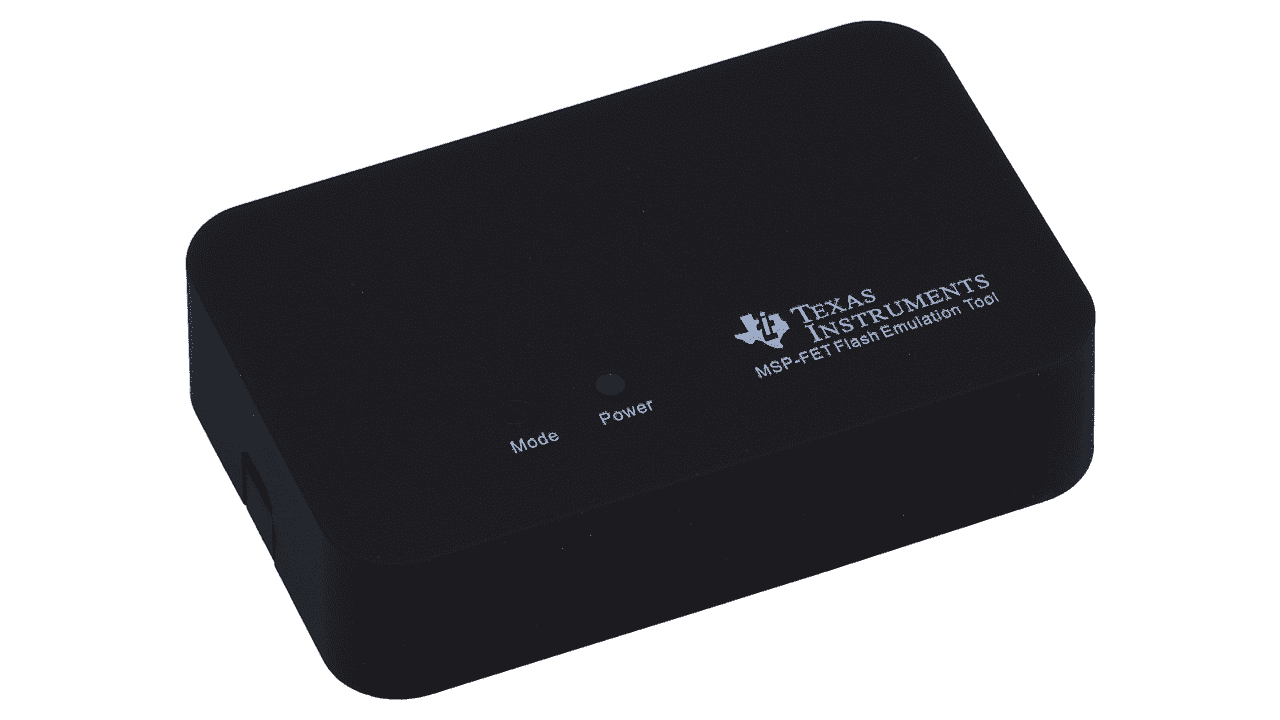
\includegraphics[width=1.0\textwidth]{../Bilder/msp_fet.png}
	\caption{Flash Emulation Tool Programmer and Debugger \Zitat{ti:MSP_FET}}
	\label{fig:msp_fet}
\end{figure}

Der MSP-FET kommuniziert mit dem MSP430-Mikrocontroller typischerweise \"uber standardisierte (Debug-)Schnittstellen wie \textbf{\Abkuerzung{Joint Test Action Group}{JTAG} (Joint Test Action Group)} oder das von Texas Instruments entwickelte \Fachbegriff{Zweidraht-Variante des JTAG-Protokolls, die Pin-Anzahl am Target reduziert und besonders f\"ur platzkritische Anwendungen von Vorteil ist.}{Spy-Bi-Wire}. (\Abkuerzung{Spy-Bi-Wire}{SBW}) \"uber diese Schnittstellen erh\"alt der MSP-FET Zugriff auf das EEM des MSP430FR5729. Wie im vorherigen \Kapitel{Hardware_VS_Software_Breakpoints} dargelegt, ist das EEM f\"ur die Realisierung von Hardware-Breakpoints zust\"andig. Der MSP-FET agiert hierbei als Vermittler, der die vom Entwickler in der \NeuerBegriff{IDE (Integrated Development Environment)} gesetzten Hardware-Breakpoint-Adressen in die entsprechenden Register des EEM schreibt und die vom EEM generierten Haltesignale empf\"angt und an die IDE weiterleitet. Somit ist der MSP-FET unerl\"asslich f\"ur die Konfiguration und Nutzung der limitierten, aber pr\"azisen Hardware-Breakpoint-Ressourcen des Mikrocontrollers. \Zitat[S. 58, Kap. 3.4]{davies:msp430}

Dar\"uber hinaus spielt der MSP-FET eine ebenso gro{\ss}e Rolle f\"ur die Implementierung und Handhabung von Software-Breakpoints. Die F\"ahigkeit, den Speicher des MSP430FR5729 (sowohl RAM als auch das beschreibbare FRAM) zur Laufzeit zu lesen und zu schreiben, ist die Grundvoraussetzung, um Instruktionen mit einer Software-Breakpoint-Routine zu ersetzen. Der Debugger liest \"uber den MSP-FET die urspr\"ungliche Instruktion an der Zieladresse aus, ersetzt diese durch eine Breakpoint-Instruktion und, nach dem Ausl\"osen des Software-Interrupts, stellt er die urspr\"ungliche Instruktion wieder her. Ferner erm\"oglicht der MSP-FET die Steuerung des Programmflusses (Anhalten, Starten, Einzelschrittbetrieb) und den Zugriff auf CPU-Register und Speicherinhalte, was f\"ur die Analyse des Systemzustands an einem Breakpoint unerl\"asslich ist. Das vom Software-Breakpoint ausgel\"oste Interrupt- oder Exception-Signal wird ebenfalls \"uber die Debug-Schnittstelle an den MSP-FET und somit an die Host-Debugger-Software gemeldet. Wie solche Hardware und Software-Breakpoints in der Entwicklungsumgebung aussehen, ist in \Abbildung{CCS_SetBR} zu sehen. Das \glqq H/W\grqq oder \glqq S/W\grqq innerhalb der eckigen Klammern steht wahlweise f\"ur \glqq Hardware\grqq oder \glqq Software\grqq welches von einem \glqq BP\grqq f\"ur \glqq Breakpoint\grqq erg\"anzt wird.

\begin{figure}[h!]
	\centering
	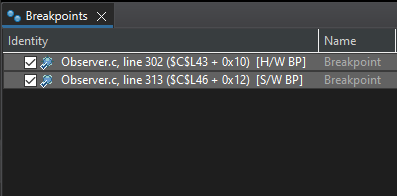
\includegraphics[width=0.75\textwidth]{../Bilder/HW_SW_Breakpoint.png}
	\caption{Code Composer Studio - Breakpoint \"Ubersicht}
	\label{fig:CCS_SetBR}
\end{figure}

\newpage
Es ist wichtig zu verstehen, dass der MSP-FET prim\"ar die Kommunikationsinfrastruktur und die Low-Level-Zugriffsmechanismen bereitstellt. W\"ahrend er das Setzen von Hardware-Breakpoints direkt \"uber das EEM steuert, stellt er f\"ur Software-Breakpoints die notwendigen Lese-, Schreib- und Kontrolloperationen zur Verf\"ugung. Die eigentliche Logik eines Software-Breakpoints – das hei{\ss}t, welche Instruktion als Breakpoint-Befehl dient, wie die urspr\"ungliche Instruktion gesichert und wiederhergestellt wird sowie der resultierende Trap behandelt wird – muss in der Debugger-Software auf dem Host und gegebenenfalls durch eine minimale Debug-Monitor-Routine auf dem Target implementiert werden, wobei der MSP-FET als Br\"ucke dient. \Zitat[S. 56, Kap. 10]{ti:slau157as, ti:slau654e}

Die Kenntnis der Funktionalit\"aten und der Arbeitsweise des MSP-FET ist somit entscheidend f\"ur die Entwicklung einer robusten Software-Breakpoint-L\"osung. Er definiert die Grenzen und M\"oglichkeiten, wie mit dem Target-System interagiert werden kann, um Breakpoints zu setzen, Zustandsinformationen abzufragen und die Programmausf\"uhrung zu steuern. Die im Folgenden zu entwickelnde Strategie zur Implementierung von Software-Breakpoints muss sich daher eng an den durch den MSP-FET und die Debug-Schnittstelle des MSP430FR5729 gegebenen Rahmenbedingungen orientieren.

%----------------------------------------------------------------------------------------------------%

\newpage
\subsection{Konzeptionierung von Software-Breakpoints}
\label{sec:KonzeptionierungSoftwareBreakpoints}

Zur Realisierung von Breakpoints existieren mehrere Ans\"atze. Ein bew\"ahrter Einstieg besteht darin, etablierte Debugger und ihre Architektur zu studieren. Im Embedded‑ und Low‑Power‑Bereich kommen beispielsweise Werkzeuge wie \NeuerBegriff{TRACE32}, \NeuerBegriff{M-Core} oder das \NeuerBegriff{MSP-FET} von Texas Instruments zum Einsatz. Diese Debugger setzen Hardware-Breakpoints \"uber spezielle Debug‑Interfaces um und bieten damit eine hohe Zuverl\"assigkeit bei minimaler Eingriffstiefe in das Laufzeitsystem.

Im Gegensatz dazu zielt die hier vorgestellte L\"osung auf eine Abwandlung der Software-Breakpoints ab, die direkt den Programmspeicher manipuliert. Dabei wird, in dieser Implementierung, an der gew\"unschten Halteadresse der originale Maschinenbefehl durch einen Sprungbefehl (Jump) ersetzt, der auf eine speziell implementierte \NeuerBegriff{Breakpoint-Handler}-Routine verweist. Beim Erreichen dieses Befehls wird zun\"achst ein kritischer Abschnitt eingeleitet: Es werden die f\"ur den Prozess relevanten Register (R1 bis R3) – namentlich \Fachbegriff{Ein Register, das die Speicheradresse des derzeitigen Befehls enth\"alt.}{Program Counter} (\Abkuerzung{Program Counter}{PC}), \Fachbegriff{Ein Register, das die Speicheradresse des letzten oder ersten Datenelements im Stack speichert.}{Stack Pointer} (\Abkuerzung{Stack Pointer}{SP}), \Fachbegriff{Register f\"ur eine Reihe von Flags, die von der arithmetisch-logischen Einheit in Abh\"angigkeit der zuletzt durchgef\"uhrten Rechenoperation gesetzt werden.}{Statusregister} (\Abkuerzung{Status Register}{SR}) und \ggf mehrere \NeuerBegriff{General-Purpose-Register (R4 bis R15)} – gesichert und Interrupts deaktiviert, um eine atomare Kontextsicherung zu gew\"ahrleisten \Zitat[S.91, Kap. 4.3]{ti:slau272d}. Anschlie{\ss}end erfolgt der \"ubergang in die Handler-Routine, die das gesamte System bis auf das Observer-Modul blockiert und so das Auslesen und Manipulieren von Speicherinhalten erm\"oglicht.

Nach der Analyse kann der urspr\"ungliche Programmzustand durch das laden der Registers\"atze wiederhergestellt werden. Eine explizite reaktivierung der Interrupts ist daher nicht n\"otig. Der Compiler stellt hierf\"ur \Fachbegriff{Compiler-spezifische, vordefinierte Funktionen, die direkt in optimierten Assemblercode umgesetzt werden.}{Compiler-Intrinsics}[Compiler-Intrinsic] bereit wie \Code{\_\_get\_SR}, \Code{\_\_get\_SP} und \Code{\_\_set\_interrupt\_state} \Zitat[S.137, Kap. 6.8.1]{ti:slau132r}. Auf diese Weise wird ein vollst\"andiger Zyklus von Unterbrechung, Inspektion und Fortsetzung des Programmflusses realisiert, ohne dass das Hauptprogramm von dem Observer-Modul tiefgreifender beeinflusst wird.

Vor diesem Hintergrund wird in den folgenden Abschnitten die Konzeptionierung erweiterter Software-Breakpoints im Detail erl\"autert und auf die daf\"ur notwendigen Voraussetzungen eingegangen.


\newpage
\subsubsection{Verwendung eines Sprungbefehls anstelle einer Trap}
\label{sec:JumpVsTrap}

Wie in \Kapitel{Hardware_VS_Software_Breakpoints} erl\"autert, basieren klassische software-Breakpoints h\"aufig auf sogenannten Trap-Instruktionen. Das Debugging-Framework der Entwicklungsumgebung unterst\"utzt dies unter anderem \"uber die \NeuerBegriff{General Extension Language} (\Abkuerzung{General Extension Language}{GEL}) – ein Makro- und Skriptsystem, das die Initialisierung von Systemen sowie die Steuerung von Debug-Sitzungen erm\"oglicht. Dar\"uber hinaus erlaubt GEL auch das Setzen von Breakpoints, Speicherzugriffe und die Ablaufkontrolle des Programms \Zitat[Kap. 7.7, 7.7.8.6 \& 7.7.8.7]{ti:CCS}.

F\"ur diese Arbeit war es jedoch erforderlich, dass bei Ausl\"osen eines Breakpoints benutzerdefinierte Routinen aus dem Observer-Modul aktiv bleiben und verwendet werden k\"onnen (\Vgl \Kapitel{Interruptgesteuertes_Lesen&Schreiben}). Diese Funktionalit\"aten sind mit dem Standardverhalten von GEL-Traps nicht kompatibel, da sie typischerweise nur auf Debugger-seitige Prozesse abzielen und keine Kontextintegration benutzerdefinierter Routinen auf dem Zielsystem erlauben.

Aus diesem Grund wurde bewusst auf die Verwendung eines Trap-Mechanismus verzichtet und stattdessen ein direkter Sprungbefehl (Jump) auf eine benutzerdefinierte Breakpoint-Handler-Routine implementiert. Dadurch wird sichergestellt, dass das Observer-Modul auch w\"ahrend einer Unterbrechung aktiv bleibt und die Kontrolle \"uber Register- und Speicherzugriffe erhalten bleibt.



\subsubsection{Implementierung erweiterter Software Breakpoints}
\label{sec:ImplementierungSoftwareBreakpoints}

Die Grundidee von Software-Breakpoints besteht darin, an einer Stelle im Programmspeicher, an der ein g\"ultiger Maschinenbefehl (\Fachbegriff{Auch op code oder operation code, ist eine meist in hexadezimaler Schreibweise angegebene Zahl, die die Nummer eines Maschinenbefehls f\"ur einen bestimmten Prozessortyp angibt.}{Opcode}) liegt, diesen tempor\"ar durch einen Sprung auf die Breakpoint-Handler-Routine zu ersetzen. Zun\"achst wird der originale Opcode gesichert, um ihn sp\"ater unver\"andert wieder einsetzen zu k\"onnen. Die Auswahl der Adresse erfordert, dass diese auf ein g\"ultiges Befehlswort ausgerichtet ist und im Stack-Bereich liegt, um Kollisionen auf das Code-Segmenten zu vermeiden. Zudem muss die Interpretation der Adresse und des zu schreibenden Sprungbefehls den aktiven Adressierungsmodus ber\"ucksichtigen.

Die Implementierung gliedert sich in folgende Schritte:
\begin{enumerate}
	\item \textbf{Adressvalidierung:} Pr\"ufen, ob die Zieladresse auf vier Byte ausgerichtet ist und im Stack liegt.
	  
	\item \textbf{Kontext-Sicherung:} In einem kritischen Abschnitt werden PC, SP, SR und alle modifizierten Register in einem Puffer abgelegt. Hierbei ist zu beachten, dass die Breite des PC vom Adressierungsmodus abh\"angt, worauf entsprechend r\"ucksicht genommen werden muss. \Zitat[S. 97, Kap. 4.4]{ti:slau272d}
	
	\item \textbf{Ersetzen des Opcodes:} Der Original-Opcode (vier Byte) wird durch den vier-Byte-Sprungbefehl (zwei Byte f\"ur den Instruction-Code, zwei Byte f\"ur die Zieladresse der Handler-Routine) \"uberschrieben. \Zitat[S.161, Kap. 4.6.2.28]{ti:slau272d}
	
	\item \textbf{Ausf\"uhrung des Breakpoint-Handlers:} Beim Eintreten des Breakpoint-Opcodes springt der PC in die Handler-Routine, die das System an weiterer Ausf\"uhrung hindert und stattdessen das Observer-Modul f\"ur weitere Debug-Schritte aktiv h\"alt.
	
	\item \textbf{Kontext-Wiederherstellung:} Nach Abschluss der Debug-Aktion werden alle Register und der urspr\"ungliche Opcode wiederhergestellt, bevor der normale Programmablauf fortgesetzt wird.
\end{enumerate}

Diese Vorgehensweise stellt die R\"uckkehr zum urspr\"unglichen Systemzustand – einschlie{\ss}lich des Originalen-Opcodes – sicher und garantiert die Konsistenz des Programms.

Um die im vorigen \Kapitel{KonzeptionierungSoftwareBreakpoints} skizzierten Konzepte robust umzusetzen, sind die im n\"achsten Abschnitt, technischen Details wie Instruktionsl\"angen und Speicher-Alignment, zu betrachten.\AI



\newpage
\subsubsection{Instruktionsl\"angen, Speicher-Alignment und Adress-Modi}
\label{sec:TechnischeUmsetzunSoftwareBreakpoints}

Die Manipulation von Befehlen im Stack ist hoch kritisch, da das Hauptprogramm keine Kenntnis vom Observer-Modul hat und eine falsche Adressierung, unterschiedlichen Adressierungs-Modi oder unvollst\"andige Opcode-substituierung zu undefiniertem Verhalten f\"uhren kann. Drei zentrale Aspekte sind dabei zu beachten:

\begin{itemize}
	\item \textbf{Speicher-Alignment:} MSP430-Instruktionen sind grunds\"atzlich an geraden Speicheradressen ausgerichtet. Vor jedem Schreib- oder Lesezugriff muss daher sichergestellt werden, dass die Zieladresse eine gerade Adresse ist. Zugriffe auf ungerade Adressen k\"onnen zu undefiniertem Verhalten f\"uhren, sofern keine Fehlerbehandlung erfolgt. Dar\"uber hinaus sind Adressen, die in der Mitte eines Opcodes liegen, ung\"ultig und d\"urfen nicht als Breakpoint oder adressiert werden.
	
	\item \textbf{Opcode-L\"angen:} W\"ahrend einzelne Maschinenbefehle in der Regel zwei bis vier Bytes belegen, k\"onnen komplexe Instruktionen – etwa \Code{CMP.B} – bis zu sechs Bytes lang sein, wie in \Abbildung{DisassemblyOpcodeLaengen} zu sehen. \Zitat[S.165, Kap. 4.6.2.32]{ti:slau272d} Diese Variabilit\"at erschwert das gezielte \"Uberschreiben von genau vier Byte, die f\"ur die Jump-Instruktion einschlie{\ss}lich Zieladresse ben\"otigt werden. Unter diesen Randbedingungen besteht die Gefahr, dass entweder zu viele oder zu wenige Bytes \"uberschrieben werden, was zu ung\"ultigen oder unbeabsichtigten Instruktionen f\"uhren kann.
	
	\begin{figure}[h!]
		\centering
		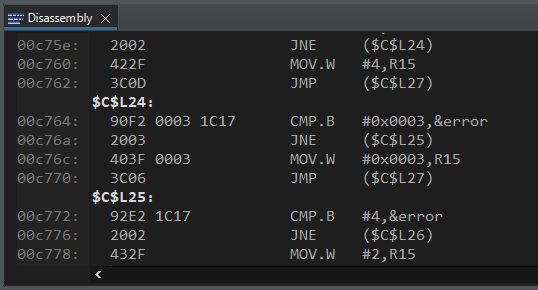
\includegraphics[width=0.7\textwidth]{../Bilder/OpcodeLaengen.png}
		\caption{Code Composer Disassembly Modus - Opcode l\"angen}
		\label{fig:DisassemblyOpcodeLaengen}
	\end{figure}
	
	\newpage
	\item \textbf{Adressierungs Modus:} Der Speicher, im Umfang von einem Megabyte, kann \"uber sieben unterschiedliche arten Adressiert werden. Wahlweise kommen 16 oder 20-Bit Adressen zum Einsatz. Diese Variabilit\"at der Adressierungsmodi und die damit einhergehenden unterschiedlichen Adressbreiten haben tiefgreifende Konsequenzen.\Zitat[S. 97, Kap. 4.4]{ti:slau272d}
\end{itemize}

Das Sichern und Wiederherstellen von Registern und des Originalen Opcodes reicht daher nicht aus, insbesondere angesichts den variablen Instruktionsl\"angen und komplexer Adressierungsmodi. 

Die gr\"o{\ss}e der Opcodes h\"angt von folgenden Parametern ab. Die Grundlegende l\"ange einer Instruktion des MSP430 liegt bei zwei Byte. Darin ist die Operation, wie beispielsweise \Code{MOV.W}, sowie die Register- und Adressierungsart kodiert. Unterschiedliche Adressierungen von Operanden \"uber Adressierungsmodi wie \glqq \Fachbegriff{Operand ist direkt in der Instruktion enthalten – also ein fester Wert, nicht aus dem Speicher.}{Immediate}\grqq , \glqq \Fachbegriff{Operand befindet sich an einer feste Speicheradresse.}{Absolute} \grqq oder \glqq \Fachbegriff{Operand ist nicht direkt gegeben, sondern steht an der Adresse, die ein Register enth\"alt.}{Indirect}\grqq, haben zur Folge, dass die Adressen oder Konstanten zus\"atzlich als \Fachbegriff{Synonym f\"ur 2 Byte gro{\ss}e Datenbreite}{Word} (2 Byte) oder \Fachbegriff{Synonym f\"ur 4 Byte gro{\ss}e Datenbreite}{extended Word} (4 Byte) kodiert werden. \Zitat[S. 97, Kap. 4.4]{ti:slau272d}

\newpage
Ein Beispiel hierzu, woraus sich der 6-Byte lange Opcode, zum Vergleichen des Speicherinhalts des Registers \glqq \&error\grqq  mit dem Hexadezimalen Wert \glqq 0x0003\grqq, aus \Abbildung{DisassemblyOpcodeLaengen} zusammensetzt: \Zitat[S. 147, Kap. 4.6.2.14 \& S. 112, Kap. 4.4.7 \& S. 108, Kap. 4.4.4]{ti:slau272d}
\\\textbf{\Code{CMP.B \#0x0003, \&error}} 
\begin{itemize}
	\item \textbf{1 Byte} Opcode f\"ur \Code{CMP.B}
	\item \textbf{1 Byte} Modus f\"ur Quell-Operand und Ziel-Operand (Immediate -> Absolute)
	\item \textbf{2 Byte} Immediate-Wert f\"ur Konstante \glqq 0x0003\grqq
	\item \textbf{2 Byte} Absolute-Adresse f\"ur Label \glqq \&error\grqq
\end{itemize}


Diese Analyse verdeutlicht die komplexit\"at der Manipulation und Wiederherstellung von Instruktionen im Stack. Eine Kopie des Stacks schafft dabei eine sichere Umgebung, in welcher der bestehende Opcode Manipuliert wird. Hierbei muss die Kopie die unterschiedlichen Adressformate und die potenziell im Stack gespeicherten, modusabh\"angigen Zeiger korrekt abbilden oder transformieren. Dies garantiert ein sicheres zur\"uckkehren in die Hauptroutinen, sowie eine Robuste Ausf\"uhrung der Funktion zum verarbeiten der \ggf mehreren Breakpoints.

Dies erschwert die Umsetzung und erh\"oht die Komplexit\"at der Routine erheblich, wodurch Timing und Konsistenz gef\"ahrdet werden. Im anschlie{\ss}enden Fazit werden die gewonnenen Erkenntnisse bewertet, offene Fragestellungen skizziert und ein Ausblick auf weiterf\"uhrende Arbeiten gegeben.

